\documentclass{article}

% if you need to pass options to natbib, use, e.g.:
%     \PassOptionsToPackage{numbers, compress}{natbib}
% before loading neurips_2019

% ready for submission
% \usepackage{neurips_2019}

% to compile a preprint version, e.g., for submission to arXiv, add add the
% [preprint] option:
%     \usepackage[preprint]{neurips_2019}

% to compile a camera-ready version, add the [final] option, e.g.:
% \usepackage[final]{neurips_2019}

% to avoid loading the natbib package, add option nonatbib:
\usepackage[nonatbib]{neurips_2019}
\usepackage{comment}
\usepackage[utf8]{inputenc} % allow utf-8 input
\usepackage[T1]{fontenc}    % use 8-bit T1 fonts
\usepackage{hyperref}       % hyperlinks
\usepackage{url}            % simple URL typesetting
\usepackage{booktabs}       % professional-quality tables
\usepackage{amsfonts}       % blackboard math symbols
\usepackage{nicefrac}       % compact symbols for 1/2, etc.
\usepackage{microtype}      % microtypography
\usepackage{bold-extra}
\usepackage{amsmath}
\usepackage{graphicx}
\usepackage{subfig}
\usepackage{array}

\title{Overparameterization, Batch Norm, and the Attack of the Confused Gradients}

% The \author macro works with any number of authors. There are two commands
% used to separate the names and addresses of multiple authors: \And and \AND.
%
% Using \And between authors leaves it to LaTeX to determine where to break the
% lines. Using \AND forces a line break at that point. So, if LaTeX puts 3 of 4
% authors names on the first line, and the last on the second line, try using
% \AND instead of \And before the third author name.

\author{%
  Zongkai Tian \\
  Department of Computer Science\\
  Columbia University\\
  116 th St & Broadway, New York, NY 10027 \\
  \texttt{zt2218@columbia.edu} \\
  % examples of more authors
  \And
   James Shin\\
   Department of Computer Science\\
   Columbia University\\
   116 th St & Broadway, New York, NY 10027 \\
  \texttt{js4785@columbia.edu} \\
  \AND
  Ruisi Wang\\
  Department of Computer Science\\
  Columbia University\\
  116 th St & Broadway, New York, NY 10027 \\
  \texttt{rw2720@columbia.edu} \\
  % \And
  % Coauthor \\
  % Affiliation \\
  % Address \\
  % \texttt{email} \\
  % \And
  % Coauthor \\
  % Affiliation \\
  % Address \\
  % \texttt{email} \\
}

\begin{document}

\maketitle
\begin{abstract}
\textit{Overparameterization}
\end{abstract}

\section{Introduction}
Neural networks have seen remarkable progress in recent years in terms of approximating complex functions using various optimization methods such as stochastic gradient descent. In particular, neural networks in practice have shown how \textit{overparameterization} (an increase in parameters of a model over the number of training data) and \textit{batch normalization}, are able to make complex neural networks easier to train. However, prior to recent research, not much was understood in terms of concretely defining why these methods work so well to speed up training. \textit{Why, precisely, do overparameterization and batch normalization allow for quicker convergence to global and local minima?} In this paper we address this question by investigating a recently-developed concept known as \textit{gradient confusion}, a measure of differences between stochastic gradients of each data sample in a training set, that causes convergence to slow down. We also will discuss overparameterization and batch normalization in-depth, which can be shown (both empirically and theoretically) to lower gradient confusion and thus speed up training.

\section{Stochastic Gradient Descent and the Definition of Gradient Confusion}
We first define gradient confusion in the context of stochastic gradient descent (SGD). Given $N$ training points $X = x_1,...,x_N$, we proceed with gradient descent, back-propagating for each training point. Using these training points, we can specify $N$ loss functions, $\{f\}_{i \in [N]}$. Then we use SGD to solve the empirical risk minimization problem; that is, we hope to find optimal solution
$$w^* = \text{arg min}_{w \in \mathbb{R}^d} \frac{1}{N} \sum_{i=1}^N f_i (w).$$
Then for iteration $k$ of the algorithm, a uniformly-random example and its loss function $\nabla \tilde{f}_k$ is used to update the weights.
$$w_{k+1} = w_k - \alpha_k \nabla \tilde{f}_k(w_k)$$

As SGD stochastically chooses a training example and performs gradient updates, on iteration $k$, the selected gradient $\nabla \tilde{f}_k$ for training example $x_k$ may very well be negatively correlated with another gradient term $\nabla f_j$ for example $x_j$. This negative correlation is said to have high \textit{gradient confusion}, a quantity introduced by Sankararaman, et al. \cite{impact}. \\

More formally, a set of objective functions $\{f_i\}_{i \in [N]}$ is said to have a $\textit{gradient confusion bound}$ $\eta \geq 0$ if, for fixed $w \in \mathbb{R}^d$,

$$ \langle \nabla f_i(w), \nabla f_j(w) \rangle \geq -\eta, \;\; \forall i \not = j \in [N]$$

That is, the inner product of the gradient vectors of every pair of unique loss functions is bounded by $-\eta$. Throughout the rest of this paper, we will use \textit{gradient confusion} to refer to the gradient inner product shown here.

\subsection{Intuition}
Intuitively, when we have a gradient confusion bound $-\eta$ that is positive, or a very small negative value, we say that there is ``low gradient confusion.'' This case would imply that an epoch of SGD over an entire dataset leads to faster training, because most of the gradient updates of the weights would have components that are aligned with each other. On the other hand, if gradient confusion bound $-\eta$ is a large negative value, we say there is ``high gradient confusion,'' which leads to slower training.

In practice, in high dimensions, \textit{randomly-chosen vectors are nearly orthogonal with high probability} \cite{Milman}; so, we might reasonably expect the \textit{average} randomly-chosen set of training examples to have approximately orthogonal gradients, as long as the number of parameters is large, and the number of training data is small, in order to minimize the probability of encountering gradient confusion. 

This may hold on expectation, but it is difficult to ensure low gradient confusion without more rigorous reasoning. We also do not have any guarantees that these gradient vectors will behave truly randomly over the course of the SGD algorithm. As such, we present general theories and guarantees of overparameterizing and batch-normalizing a network, as well as empirical experiments, in order to show that low gradient confusion indeed holds. This analysis would then concretely explain why training is sped up when these methods are employed, and also hopefully shed light into how methods can be designed in order to speed up training, which is an incredibly expensive task.

\subsection{The effect of network layer width on gradient confusion}
Consider a simple two-layer linear network $g(\textbf{x}) = \textbf{W}_1 \textbf{W}_0 \textbf{x}$, with $\textbf{x} \in \mathbb{R}^d$, $g(\textbf{x}) \in \mathbb{R}$, $\textbf{W}_1 \in \mathbb{R}^{l \times d}$, and $\textbf{W}_0 \in \mathbb{R}^{1 \times l}$. Also, suppose element $w_{ij} \stackrel{}{\sim} \text{Normal}(0, 1/l)$, $\forall w_{ij} \in \textbf{W}_0, \textbf{W}_1$, and also $x_i \in \textbf{x} \stackrel{}{\sim} \text{Normal}(0, 1/d)$. Chen, et al. \cite{chen} provides the following bounds for expected value and variance of the inner product:
$$\mathbb{E}_{\textbf{W}, \textbf{x}}[\langle \nabla f_i, \nabla f_j \rangle] = \Theta(\frac{1}{l}), \;\; \forall x_i, x_j$$
$$\text{var}_{\textbf{W}, \textbf{x}}(\langle \nabla f_i, \nabla f_j \rangle) \leq \mathbb{E}_{\mathbf{W}, \mathbf{x}} [||\nabla f_i||^2 ||\nabla f_j||]^2 = O(\frac{1}{l^2})$$

\begin{figure}[h]
	\centering
    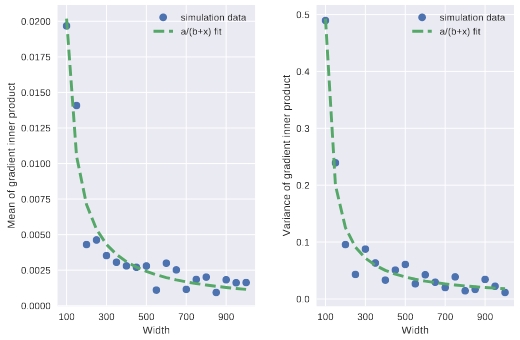
\includegraphics[width=0.5\textwidth]{pics/overparameterization/grad_inner_prod_exp_var.png}
	\caption{Simulation by Sankararaman et al. \cite{gradient_confusion} showing the mean and variance of gradient inner products for linear neural networks.}
	\label{fig:mean_inner_prod}
\end{figure}

This implies that width $l$ and gradient confusion have an inverse relationship. The proof can be found in the appendix of Chen, et al. \cite{chen}. The paper also showcases experiments of which we abbreviate here in Fig. \ref{fig:mean_inner_prod}, showcasing the relationship between network width and gradient confusion. They used a fully-connected 5-layer linear neural network of input dimension $d = 100$, where each layer took on the width specified in the graph. Both mean and variance of the gradient inner products decrease at a rate of $O(1/l)$, thus verifying the bounds above.

We can now directly apply Chebyshev's inequality to their result get our own more precise understanding of the implications behind these bounds:
$$\boxed{\mathbf{P}\left( \left\lvert \langle \nabla f_i, \nabla f_j \rangle - \Theta(\frac{1}{l}) \right\rvert \geq \epsilon  \right) \leq \frac{1}{\epsilon^2}O(\frac{1}{l^2}), \;\; \forall i \not = j \in [N]}$$
As width $l$ of the middle layer is increased, terms $\Theta(1/l)$ and $O(1/l^2)$ approximate to zero. This shows that the probability of the inner product of any two gradients of the losses deviating greatly from zero is very small. That is, as the width increases, the gradient inner products concentrate more towards zero, and therefore become more deterministic; this deterministic behavior of gradients with width overparameterization agrees with the findings of other works \cite{oymak}, \cite{bassily}, \cite{SimonDu}.\\

As such, overparameterizing a network by increasing width certainly reduces gradient confusion, thus leading to faster training time. In order to precisely understand why this is the case from an optimization point of view, we dive deeper into work by S. Du, et al \cite{SimonDu}. which discusses how gradient descent can provably optimize overparametrized networks.

\section{Over-parameterization}
We survey previous research work on optimization and generalization aspects of two-layer neural networks, which mainly focus on how they converge to global minimum and generalize in the over-parameterized setting. To investigate convergence guarantees to global minima, and study about speed of convergence, we focus on Paper \cite{SimonDu} by S.Du which talks about how over-parameterization makes Gram matrix (H(x)) remains positive definite and holds a lower bounded least eigenvalue that guarantees the linear convergence to global minima. Paper \cite{SoudryCarmon} by Soundry and Carmon discuss by analyzing the properties of differentiable local minima (DLMs) of the mean square error (MSE) for mild over-parameterization, it guarantees zero training loss for single hidden layer and multiple hidden layers cases. Paper \cite{Arora} by Arora refines the analysis of paper \cite{SimonDu} with a larger width and prove why true labels will convergence faster than random labels. And it also discussed about generalization bounds, while papers \cite{Weinan1} and \cite{Weinan2} by Weinan have a further discussion about generalization bounds. 

For the experiment part, we refer to Paper  \cite{SimonDu} by varying different width to prove that over-parameterization can significantly improve the converge rate, other aspects. Then we set up our own experiment to reproduce but with much more neurons to see the pattern from a different view. 

\subsection{Convergence to Global Minima}
In Paper\cite{SimonDu}, it addresses that for an non-convex and non-smooth optimization objective function, even with random labels, with the randomly initialized first-order methods such as stochastic gradient descent, it can still guarantee to converge to zero training loss and find global minimums.\\

The theory part separates the discussion with continuous time analysis and discrete time analysis.And we are going to mainly focus on continuous time analysis part for theorem proofs. To set the foundation for the discussion, it firstly define the concept of gradient flow, which represents gradient descent with infinitesimal steps. To represent in a mathematical way:
\begin{center}
    $\frac{d W_r(t)}{dt} = -\frac{\partial L(w(t),a)}{\partial W_r(t)}$
\end{center}

The main theorem for the convergence rate of gradient flow has four mean assumptions, which can be addressed as below:
\begin{itemize}
\item No two inputs are parallel and Gram matrix $H(x)$ has a positive minimum eigenvalue.
\item Scaled data:$\|x_i\|_{2} = 1$ and $|y_i|\leq C$. As noted,these assumptions are only for simplification and also put in a bounded label to match with most real world data set.  
\item Over-parameterization :$m=\Omega(\frac{n^6}{\lambda^4_0 \sigma^3})$
\item Random initialization: $W$ i,i,d initialize $w_r\sim N(0,I),\ a_r \sim unif[{-1,1}]$
\end{itemize}

\text{for}$\ r\in [m]$, then with probability at least $1-\sigma$ over the initialization, we have 
\begin{center}
    $\|u(t)-y\|^2_2 \leq exp(-\lambda_0 t)\|u(0)-y\|^2_2$
\end{center}

What this theorem shows is that if m is large enough, the training error can be guaranteed that it will converge to 0 with a linear rate. 

For the proof of this theorem, there are four lemmas to explain how the conclusion come out step by step. Firstly with arc-consine kernels and law of the large numbers. It is not hard to show that Gram matrix $H_{ij}(t)$ satisfied the function:
\begin{center}
    $H_{ij}(t) = \frac{1}{m} x_i^T x_j\sum_{r=1}^{m}\Pi\left\{ x_i^T w_r(t)\geq 0,x_j^T w_r(t)\geq 0\right\}$
\end{center}
And if m is large enough, it makes the initial random state close to rates during the training ($W(t)\approx W$). And then $H(t) \approx H(0) \approx H^{\infty}$. In that case, the derivative of predicted value can be written as 
\begin{center}
    $\frac{d u(t)}{dt} = H(t)(y-u(t)) \approx H^{\infty}(y-u(t))$
\end{center}
With all these foundations addressed above, then in lemma 1 it shows $H(0)$ and $H^{\infty}$ are close based on the Law of Large Numbers and $H(0)$ has a lower bounded least eigenvalue with high probability. Lemma 2 makes a further step and points out that If weights $w_r(t)$ is stable, $H(t)$ is close to $H^{\infty}$ as well. Lemma 3 started to show with the least eigenvalue of $H(t)$ is lower bounded, the loss will converges at a linear convergence rate as well as weights at t will be close to the initialization one. Lemma 4 broadcasts the lemma 3 to a wider realm R to fit in all t. \\ 

Similar to continuous time analysis, discrete time analysis
also comes to the conclusion that with probability at least $1-\sigma$ over the initialization, we have 
\begin{center}
    $\|u(t)-y\|^2_2 \leq (1-\frac{\eta \lambda_0}{2})^k\|u(0)-y\|^2_2$
\end{center}
\\
In Paper\cite{Arora}, it refines the analysis of Paper \cite


\\

\subsection{Experiments}

In Paper\cite{SimonDu},by using synthetic data, experiments in the paper has uniformly generates $n = 1000$ data points from a $d = 1000$ dimensional unit sphere and generate labels from a one-dimensional standard Gaussian distribution. 
Run 100 epochs of gradient descent with different widths $m$.Figure \ref{fig:convergerate} shows how different m affects the convergence rates. As m becomes lager, it has a better convergence rate.

\begin{figure}[h]
	\centering
    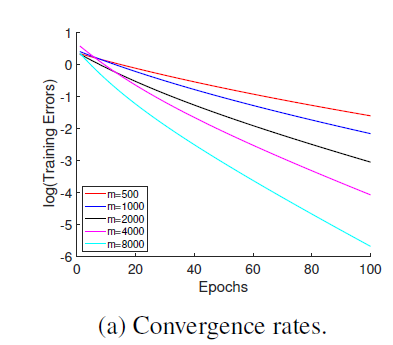
\includegraphics[scale= 0.5]{pics/overparameterization/ConvergeRate.PNG}
	\label{fig:convergerate}
\end{figure}

Figure \ref{fig:patternsample} tests the relation between different m and the number of pattern changes.
\begin{figure}[h]
	\centering
    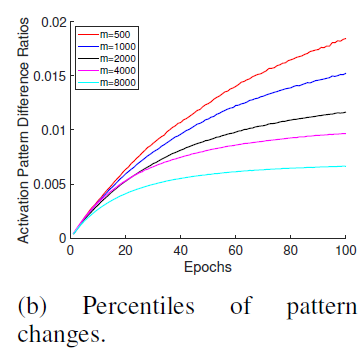
\includegraphics[scale= 0.5]{pics/overparameterization/PatternSample.PNG}
	\label{fig:patternsample}
\end{figure}

Figure \ref{fig:maxdistance} tests the relation between different m and maximum distances between wights vectors and their initialization.
\begin{figure}[h]
	\centering
    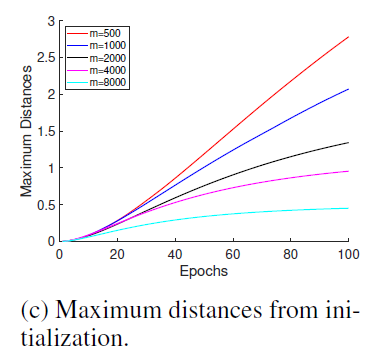
\includegraphics[scale= 0.5]{pics/overparameterization/maximumdistance.PNG}
	\label{fig:maxdistance}
\end{figure}

So generally with over-parameterization m becomes larger, convergence rate is better;the percentiles of pattern changes and the maximum distance from the initialization become smaller.
\\

We did our own experiments referring to Paper\cite{SimonDu} result.The experiment uses synthetic data, with $X$ from random generator $n = 10$ data points, and $d = 1000$ dimensional unit sphere. It runs with $m = 100000$ neurons.$y$ labels from a one-dimensional standard Gaussian distribution.

In Figure \ref{fig:zeroloss}, it shows when $m$ is large enough, the training loss will converge to 0 even with random labels. 

\begin{figure}[h]
	\centering
    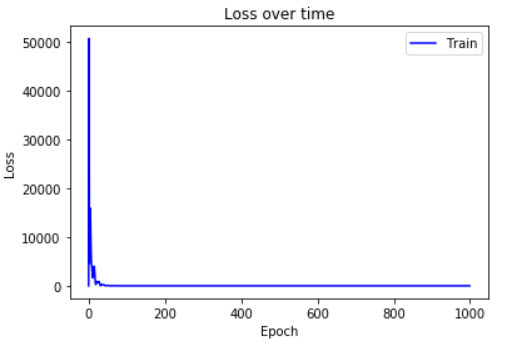
\includegraphics[scale = 0.5]{pics/overparameterization/loss_over_time_0-1k.jpg}
	\label{fig:zeroloss}
\end{figure}


On the top of graph Figure\ref{fig:zeroloss} result, Figure\ref{fig:twohundredloss} shows the convergence rate is generally fast with not too much epochs required with over-parameterization. 

\begin{figure}[h]
	\centering
    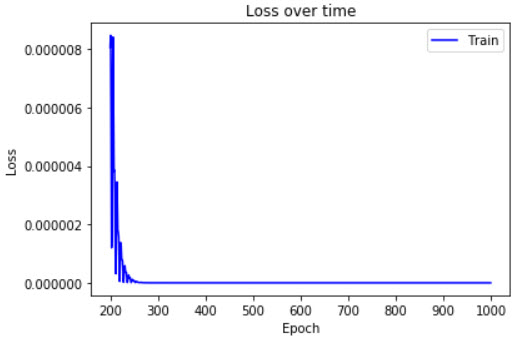
\includegraphics[scale = 0.5]{pics/overparameterization/loss_over_time_200-1k.jpg}
	\label{fig:twohundredloss}
\end{figure}

In addition, \ref{fig:maxdistanceloss}  tests on the maximum of the distances between updated weight vector and its initialized value  with a large m, the distance converges with increased epochs and converges pretty fast. 

\begin{figure}[h]
	\centering
    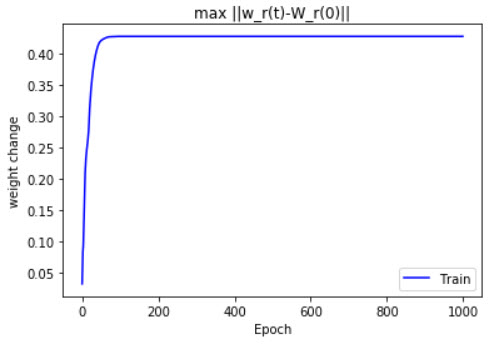
\includegraphics[scale = 0.5]{pics/overparameterization/max_weight_change.jpg}
	\label{fig:twohundredloss}
\end{figure}

\\
\subsection{Fine-Grained Analysis of Optimization and Generalization for Overparameterized Tow-layer Neural Networks}
Previous works shows that sufficiently powerful nets(with vastly more parameters than number of training samples) can attain zero training error, regardless of whether the data is properly labeled or randomly labeled.The gradient descent can allow an overparameterized multi-layer net to attain arbitrarily low training error on fairly generic datasets.

This paper accurately estimate the magnitude of training loss in each iteration. The key finding is that the number of iterations needed to achieve a target accuracy depends on the projections of data labels on the eigenvectors of a certain Gram matrix. Also, it give a generalization bound for the solution found by GD, based on accurate estimates of how much the network parameters can move during optimization. The generalization bound depends on a data-dependent complexity measure and notably, is completely independent of the number of hidden units in the network.

As to Generalization bounds, the well known VC-dimension of neural networks is at least linear in the number of parameters and therefore classical VC theory cannot explain the generalization ability of modern neural networks with more parameters than training samples. PAC-Bayes approach to compute non-vacuous generalization bounds for MNIST and ImageNet, respectively. All these bounds depend on certain properties of the trained neural networks. In the paper, one of main results shows :

For any 1-Lipschitz loss function, the generalization error of the two-layer ReLU network found by GD is at most 
\begin{center}
  $\sqrt{\frac{2y^T(H^\infty)^-1y}{n}}$
\end{center}
In that case, fix an error parameter $\epsilon > 0$ and failure probability $\sigma \in (0,1)$ Suppose we have data $S={(x_i,y_i)}_{i=1}^n$ are i.i.d. samples from $a (\lambda_0,\frac{\sigma}{3},n)$ - non-degenerate distribution D, and $k = O(\frac{\epsilon\lambda_0\sigma}{\sqrt{n}}$,$m \geq K^{-2}poly(n,\lambda_0^{-1},\sigma^{-1},\epsilon^{-1})$.Consider any loss function $l:R*R ->[0,1]$ that is 1-Lipschitz in the first argument such that $l(y,y)=0 $Then with probability at least $1-\sigma$ over the random initialization and training examples, the two-layer neural network $f_{w(k),a}$ trained by GD for $k\geq\omega(\frac{1}{\mu^{\lambda_0}}\log{\frac{1}{\sigma_\epsilon}})$ iterations has population loss $L_D(f_{W(k),a})= E_{(x,y)~D}[l(f_{W(k)},a(X),y)]$ bounded as
\begin{center}
    $L_D(f{W(k),a})\leq \sqrt{\frac{2y^T(H^\infty)^-1y}{n}} +3\sqrt{\frac{\log(\frac{6}{\sigma}}){2n}}+\epsilon$
\end{center}
\subsection{A Priori Estimates For Two-layers Neural Networks}
We provide a perspective for understanding why two-layer neural networks perform better than kernel methods. We focus on two -layer networks, and we consider models with explicit regularization. We establish estimates for the population risk which are symptotically sharp with constants depending only on the properties of the target function. 
\begin{itemize}
\item We establish a priori estimates of the population risk for learning two -layer neural networks with an explicit regulation. 
\item We make a detailed comparison between the neural network and kernel methods using these a priori estimates. 
\end{itemize}

For a two-layer neural network $f(x;\theta)$ of width m, we define the regularized risk as 
\begin{center}
  ${\MakeUppercase{J}_\lambda}(\theta) : = \hat{\MakeUppercase{L}_n}(\theta)+ \lambda(\|\theta\|_P+1)$
\end{center}
The +1 term at the right hand side is included only to simplify the proof. Our result also holds if we do not indclude this term in  the regularized risk. The corresponding regularized estimator is defined as 
\begin{center}
  $\hat{\theta_{n,\lambda}} = argmin{{\MakeUppercase{J}_\lambda}(\theta)}$
\end{center}

For any $f \in barron space(\omega)$,there exists a two-layer neural network $f(x;\hat{\theta}$ of width m with $\|\Hat{\theta}_P\leq 2\gamma_2(f)$, such that
\begin{center}
  $E_x[(f(x)-f(x;\Hat{\theta}))^2]\leq\frac{3\gamma_2^2(f)}{m}$
\end{center}
The basic intuition is that the integral representation of f allows us to approximate f by the Monte-Carlo method:$f(x) \approx\frac{1}{m}\sum_{k=1}^{m} a(w_k){\sigma(<w_k,x>)}$ where${W_k}_{k=1}^m$ are sampled from the distribution $\pi$

The main result shows 
\begin{itemize}
\item For noiseless case, Assume that the target function $f^* /in B_2(\omega)$ and $\lambda \geq \lambda_n$. Then for any $\sigma > 0 $ and, the probability at least $1-\sigma$ over the choice of the training set $S$, we have
    \begin{center}
      $E_x[(f(x;\Hat{\theta})-f^*(x))^2]\leq\frac{\gamma_2^2(f^*)}{m} +\lambda \Hat{\gamma_2}(f^*)+\frac{1}{\sqrt{n}}(\Hat{\gamma_2}(f^*)+\sqrt{\ln{\frac{n}{\sigma}}})$
    \end{center}
And the population risk for the kernel methods should be much larger than the population risk for the neural network.
\item For noisy case, Assume that the target function $f^* /in B_2(\omega)$ and $\lambda \geq \lambda_n$. Then for any $\sigma > 0 $ and, the probability at least $1-\sigma$ over the choice of the training set $S$, we have
      $E_x[(f(x;\Hat{\theta})-f^*(x))^2]\leq\frac{\gamma_2^2(f^*)}{m} +\lambda B_n \Hat{\gamma_2}(f^*)+\frac{B^2_n}{\sqrt{n}}(\Hat{\gamma_2}(f^*)+\sqrt{\ln{\frac{n}{\sigma}}})+\frac{B^2_n}{\sqrt{n}}(c_0 \sigma^2+\sqrt{\frac{E[\xi^2]}{n^{1/2}\lambda}})$
\item For classification problem, under the same assumption as above, and taking $\lambda = \Lambda_n$, for any $\sigma \in (0,1)$, with probability at least $1-\sigma$, we have
    \begin{center}
      $\epsilon(\Hat{\eta}) \leq \epsilon(\eta ^*) + \frac{\gamma_2^2(f^*)}{\sqrt{m}}+\Hat{\gamma^{1/2}}(f^*)\frac{\ln^{1/4}{d}+\ln^{1/4}{\frac{n}{\sigma}})}{n^{1/4}}$
    \end{center}
\end{itemize}

And for numerical experiments, it has been tested from three aspects:
\begin{itemize}
\item Shape bounds for the generalization gap.

The test accuracy of the regularized and unregularized solution are generally comparable, but the values of $\frac{\|\theta\|_P}{\sqrt{n}}$ are different. Especially, the values of the unregularized models are always several orders of magnitude larger than that for the regularized models.

Also, by comparing of the path norms between the regularized and un-regularized solutions for varying widths, it shows for the un-regularized model this quantity increases with network width, whereas for the regularized model it is almost constant. 
\item Dependence on the Initialization.
By testing on $m=10000,n= 100$ and vary the variance of the random initialization $K$, it shows regularized models are much more stable than the un-regularized models. 
\end{itemize}

\subsection{A Comparative Analysis of the Optimization and Generalization Property of Two-layer Neural Network and Random Feature Models Under Gradient Descent Dynamics}

Firstly, it prove that the results of Simon Du still hold, the gradient descent dynamics still converges to a global minimum exponentially fast, regardless of the quality of the labels. And functions obtained are uniformly close to the ones found in an associated kernel method, with the kernel defined by the initialization. Secondly, it prove that for target functions in the appropriate reproducing kernel Hilbert space (RKHS), the generalization error can be made small if certain early stopping strategy is adopted for the gradient descent algorithm. The conclusion can be explicit regularization is necessary for two-layer neural network models to fully realize their potential in expressing complex functional relationships. 

The problem has been set up with the regression problem with a training data. By fitting into a two -layer neural network, the ultimate goal is to minimize the population risk and in practice, it can only work with the following empirical risk. 

To analyse the over-parameterized case, the paper has demonstrated in four aspects:
\begin{itemize}
\item properties of the initialization 
For any fixed $\sigma > 0$,with probability at least $1-\sigma$ over the random initialization, we have
    \begin{center}
      $\Hat{R_n}(\theta_0)\leq {1\2}(1+c(\sigma)\sqrt{m}\beta)^2$
    \end{center}
where $c(\sigma) = 2+\sqrt{\ln{\frac{1}{\sigma}}}$.

\item Gradient descent near the initialization 
For any fixed $\sigma \in (0,1)$, assume that $m \geq \frac{8}{\lambda_n^2}\ln(\frac{2n^2}{\sigma})$.Then with probability at least $1-\sigma$ over the random choices of $\theta_0$, we have the following holds for any $t\in[0,t_0]$,
    \begin{center}
      $\Hat{R_n}(\theta_t)\leq e^{-m(\lambda_n^{(a)}+\beta^2\lambda_n^{(b)})}t\Hat{R_n}(\theta_0)$
    \end{center}
    
\item Characterization of the whole GD trajectory
\item Curse of dimensionalality pf the implicit regularization
\end{itemize}

The numerical results to illustrate our theoretical analysis with two tests: 
\begin{itemize}
\item The first experiment studies the convergence of GD dynamics for over-parameterized two-layer neural networks with different initialization. GD algorithm for the neural network models converges exponentially fast for all initialization considered.
\item The second experiment compares the GD dynamics of two -layer neural networks and random feature models. When the width is very small, the GD algorithm for the random feature model does not converge, while it does converge for the neural network model and the resulting model does generalize. For the intermediate width, the GD algorithm for both models converges, and it converges faster for the neural network model than for the random feature model. The test accuracy is slightly better for the resulting neural network model. When width is large, the behavior of the GD algorithm for two models is almost the same. 
\end{itemize}

This paper has shown that for over-parametrized two-layer neural networks without explicit regularization, the gradient descent algorithm is sufficient for the purpose of optimization. But to obtain dimension-independent error rates for generalization, one has to require that the target function be in the RKHS with a kernel defined by the initialization. Given a target function in the Barron space, in order for implicit regularization to work, one has to know before hand that kernel function for that target function and use that kernel function to initialize the GD algorithm. This requirement is certainly impractical. In the absence of suck a knowledge, one should expect to encounter the curse of dimensionality for general target function in Barron space, as is proved in this paper. 

\section{BatchNorm}
\label{label:BatchNorm}

\subsection{Architecture of Batch Normalization}


Ioffe \& Szegedy \cite{batchnorm} originally proposed that adding batch normalization (BatchNorm) as part of the network architecture. The new BatchNorm network achieves the same accuracy on a state-of-the-art image classification model with 14 times faster.

BatchNorm is applied at each neuron individually. Figure \ref{fig:batchnorm} shows how it works on a fully-connected network. 


\begin{figure}[h]
	\centering
    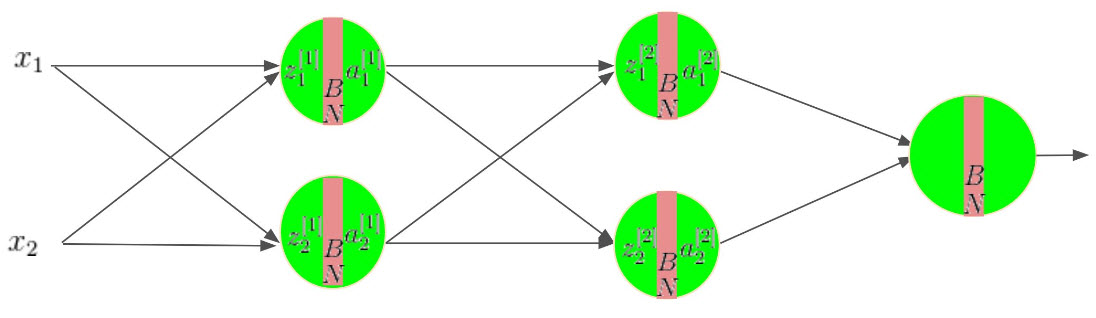
\includegraphics[width=\textwidth]{pics/batchNorm/batch-normalization.jpg}
	\caption{Batch Normalization Architecture\\Source: https://www.learnopencv.com/batch-normalization-in-deep-networks/}
	\label{fig:batchnorm}
\end{figure}

\subsection{Train with Batch Normalization}
In an un-normalized network, for neuron $i$ at an arbitrary layer, $z_i=w_ix$ and $a_i=g(z_i)$ where $x\in\mathcal{R}^{d\times m}$ is a mini-batch of size $m$ $d$-dimensional input into the neuron (it could be training data or output from previous layer) and $g$ is a non-linear activation function. So $z_i$ is vector of size $m$. Bias term $b$ and layer index is omitted for simplicity. BatchNorm is added in each neuron as the brown slice shown in Figure \ref{fig:batchnorm} before non-linear activation. On each individual neuron, we calculate:

\begin{align*}
    z_i^{norm}& = \frac{z_i-\mu}{\sqrt{\sigma^2+\epsilon}}  &(1)\\
    \hat{z}_i&= \gamma_i\cdot z_i^{norm}+\beta_i  &(2)\\
    a_i&=g(\hat{z}_i) &(3)
\end{align*}

In above equations, $\gamma_i$ and $\beta_i$ are a pair of introduced parameters that to be learned. $\mu$ and $\sigma^2$ are mean and variance of the mini-batch $z_i$, respectively. They then scale and shift the normalized value $z_i^{norm}$ to ensure that the not all transformed data fall under the linear regime of non-linear activation. $\epsilon$ is added for numerical stability of the calculation (typical value is $10^{-8}$). Note that at each step of mini-batch training, the mean and variance of $z_i$ need to be recalculated.

\subsection{Gradient Descent of Batch Normalization}

During training phase, the chain rule is still applicable to a BatchNorm network. For an arbitrary loss function $l$, the chain rule is as follows:

\begin{align*}
   \frac{\partial l}{\partial z_i^{norm}} &= \frac{\partial l}{\partial \hat{z}_i}\cdot\gamma_i\\
   \frac{\partial l}{\partial \sigma^2}  &= \sum_{i=1}^m\frac{\partial l}{\partial z_i^{norm}}\cdot(z_i-\mu)\cdot\frac{-1}{2}(\sigma^2+\epsilon)^{-3/2} \\
   \frac{\partial l}{\partial \mu}  &= \sum_{i=1}^m\frac{\partial l}{\partial z_i^{norm}}\cdot \frac{-1}{\sqrt{\sigma^2+\epsilon}}\\
   \frac{\partial l}{\partial z_i}  &=  \frac{\partial l}{\partial z_i^{norm}} \cdot\bigg(\sqrt{\sigma^2+\epsilon}\bigg)^{-1} + \frac{\partial l}{\partial \sigma^2}\cdot\frac{2(z_i-\mu)}{m} +  \frac{\partial l}{\partial \mu}\cdot\frac{1}{m}\\
   \frac{\partial l}{\partial \gamma_i}  &=  \sum_{i=1}^m\frac{\partial l}{\partial \hat{z}_i}\cdot z_i^{norm} \\
   \frac{\partial l}{\partial \beta_i}  &= \sum_{i=1}^m\frac{\partial l}{\partial \hat{z}_i} \\
\end{align*}

Therefore, we can still use backpropagation to update all the parameters in a BatchNorm neural network.

\subsection{Inference with Batch Normalization}

Suppose the whole training data are split into $B$ mini-batches. When inference with BatchNorm network, deterministic mean and variance, $\mu$ and $\sigma^2$ in Eq. (1) independent of mini-batch are desired. To achieve a fixed mean and variance, once training is completed, with frozen parameters, the $B$ training mini-batches are re-processed through the trained network. Then for neuron $i$, the mean for mini-batch $k\in\{1,2,\cdots,B\}$ is denoted as $\mu_k$ and the variance as $\sigma^2_k$. Then let

\begin{align*}
   M &= \frac{1}{B}\sum_{k=1}^B\mu_k\\
   V &= \frac{m}{m-1}\Bigg(\frac{1}{B}\sum_{k=1}^B\sigma^2_k\Bigg)\\
\end{align*}

, where $M$ is the average of the means of mini-batches and $V$ is unbiased estimate of the average variance of mini-batches. Therefore, when doing inference on test data, Eq. (1) is rewritten as:

\begin{align*}
    z_i^{norm}& = \frac{z_i-M}{\sqrt{V+\epsilon}}
\end{align*}


\subsection{Loss-Landscape Smoothing} \label{landsmooth}
In paper \cite{landscape} they show that landscape of loss function is smoother in BatchNorm network. BatchNorm reduces effective Lipschitzness constant and improve smoothness of the gradient.

\subsubsection{Observations}

In this paper \cite{landscape}, they perform experiments with two deep architectures to observe, a VGG-type convolutional network with 11-19 layers (exact number of layers is not specified in the paper) on CIFAR10 dataset and a 25-layer deep linear network (DLN) on synthetic Gaussian data. They also explicitly add time-varying noise of non-zero mean and non-unit variance to each batch-normalized node independently (referred as "noisy" BatchNorm model in the paper) so that distribution of activation on each node in a mini-batch is ensured to be unstable. From the performance of VGG network, shown in Figure \ref{fig:vgg}, they observe BatchNorm and noisy BatchNorm have comparable performance, they both converge faster than standard "vanilla" network. However, Figure \ref{fig:vgg} shows that although "noisy" BatchNorm achieved faster training speed than standard "vanilla" network and comparable performance as BatchNorm, the weight distribution of "noisy" BatchNorm  is more noisy than the standard one which indicate a large ICS as defined in Ioffe \& Szegedy, 2015 \cite{batchnorm}. Also, notice that in Layer \#13 the weight distribution of BatchNorm has more ICS than standard network.

\begin{figure}[h] 
	\centering
    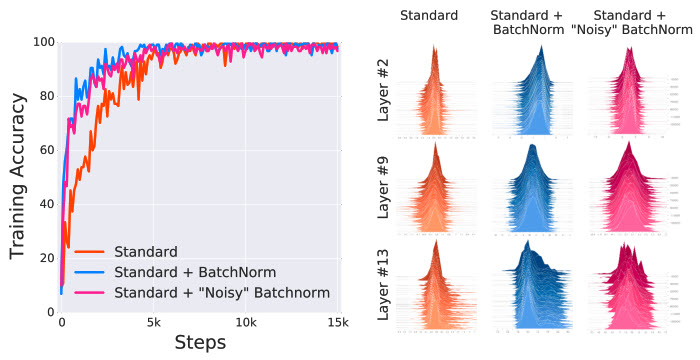
\includegraphics[scale=0.6]{pics/batchNorm/Santurkar_fig2.jpg}
	\caption{VGG Performance}
	\label{fig:vgg}
\end{figure}

The above findings is hard to align with what is claimed in Ioffe \& Szegedy, 2015  \cite{batchnorm} that BatchNorm helps stabilize internal weight distribution so to reduce ICS. To investigate why is the case that BatchNorm improve training process, they analyze the optimization landscape in VGG networks and show it in Figure \ref{fig:optimizationlandscape}.

\begin{comment}
To further quantify the findings, a broader notation of ICS of activation i at time t is defined as $||G_{t,i}-G^{'}_{t,i}||_2$ in the paper (Santurkar, 2018), where
\begin{align*}
	G_{t,i}&=\nabla_{W_{i}^{(t)}}\mathcal{L}(W_{1}^{(t)},\cdots,W_{k}^{(t)};x^{(t)},y^{(t)})\\
	G^{'}_{t,i}&=\nabla_{W_{i}^{(t)}}\mathcal{L}(W_{1}^{(t+1)},\cdots,
	W_{i-1}^{(t+1)},W_{i}^{(t)},W_{i+1}^{(t)},\cdots,W_{k}^{(t)}
	;x^{(t)},y^{(t)})
\end{align*}

In above definition, $W_{1}^{(t)},\cdots,W_{k}^{(t)}$ are weights of each of the $k$ layers at time $t$. $G_{t,i}$ is the gradient of the loss before applying any weights update and $G^{'}_{t,i}$ is the gradient after updating the first $i-1$ layers. So, $l_2$ difference of $G$ and $G'$ corresponds to the change in the optimization landscape of $W_i$ caused by its input change.

\begin{figure} 
	\centering
    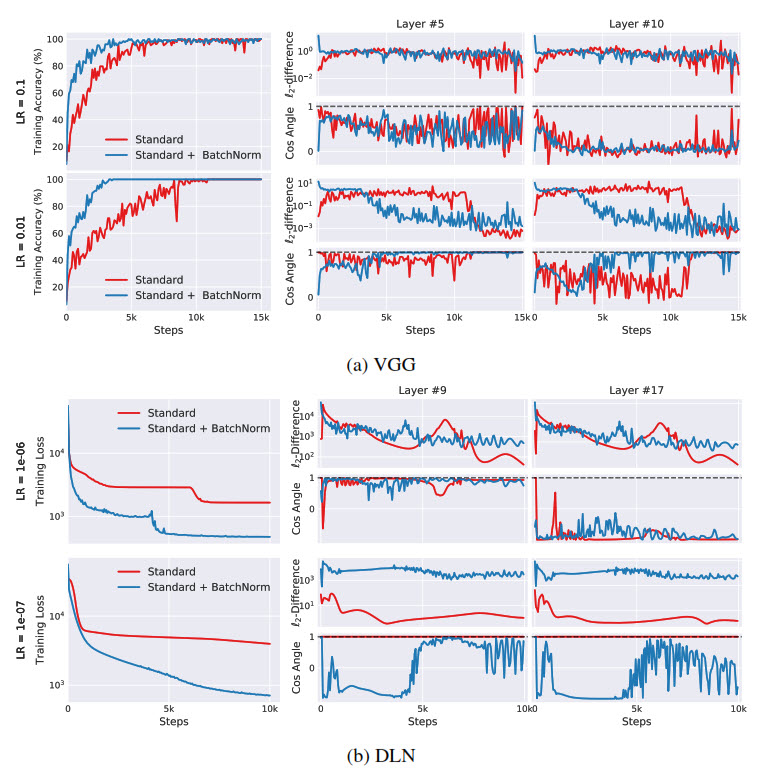
\includegraphics[width=\textwidth]{pics/batchNorm/Santurkar_fig7.jpg}
	\caption{ICS}
	\label{fig:ICSshift}
\end{figure}

Regardless of the difference in definition, they measure cosine angle (ideal value is 1) and $l_2$-difference (idea value is 0) of the gradients and plot it in Figure \ref{fig:ICSshift}. They claim that the figure shows that BatchNorm does not clearly improve ICS. DLN has even worse ICS with BatchNorm.
\end{comment}

\subsubsection{Theory Results}
At each training step, suppose the weights is at position A of the optimization landscape, they calculate the gradient at position A, then they "walk" in the gradient direction of A and mark some positions along the way. In graph (a) of Figure \ref{fig:optimizationlandscape}, shaded area is the change in loss between A and each of the marked positions. In graph (b) the shaded area is $l_2$-difference of the gradient at A and the gradient at each of the marked positions. Graph (c) shows the maximum value of gradient difference (as $l_2$-norm) divided by distance from A to corresponding marked position. The maximum value can be seen as "effective" Lipschitz constant. It is evident that BatchNorm improves smoothness of the optimization landscape.

\begin{figure}[h]
	\centering
    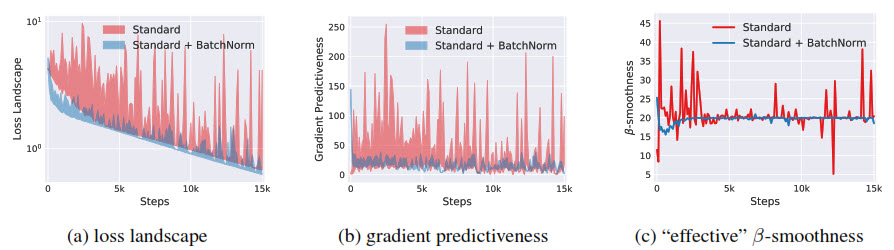
\includegraphics[width=\textwidth]{pics/batchNorm/Santurkar_fig4.jpg}
	\caption{Optimization Landscape}
	\label{fig:optimizationlandscape}
\end{figure}

In following section, they analyze the phenomenon theoretically. In the theoretical setup, a single BatchNorm layer is arbitrarily inserted at a fully-connected layer. Layer weights are denoted as $W_{ij}$. An arbitrary unnormalized loss function at current layer as $\mathcal{L}$ and normalized loss $\hat{\mathcal{L}}$ that could have downstream non-linear layers. For input $x$ let $y=Wx$. $\hat{y}=\text{BN}(y)$ is batch-normalized $y$ that has mean 0 and variance 1. Then $z=\gamma\hat{y}+\beta$ where $\gamma$ and $\beta$ are assumed to be constant for the following analysis. 

\textbf{Theorem 4.1} shows that BatchNorm improve Lipschitzness of the loss with respect to $y_j$.

\begin{align*}
	||\nabla_{y_j}\hat{\mathcal{L}}||^2&\leq\frac{\gamma^2}{\sigma^2_j}\bigg(||\nabla_{y_j}\mathcal{L}||^2
	- \frac{1}{m} \langle \mathbf{1},\nabla_{y_j}\mathcal{L} \rangle^2 
	- \frac{1}{m}\langle \nabla_{y_j}\mathcal{L}, \hat{y}_j \rangle^2 \bigg)\\
\end{align*}

, where $\sigma_j^2$ is variance of a batch of outputs $y_j\in\mathrm{R}^m$ and $j$ denotes an arbitrary node in the normalized layer. 

The value of $\sigma_j^2$ tends to be large in practice. The inequality utilizes an assumption that $\partial \hat{\mathcal{L}}/\partial z_j = \partial \mathcal{L}/\partial y_j$. The second term, $ \langle \mathbf{1},\nabla_{y_j}\mathcal{L} \rangle^2=\big( \sum_{k=1}^{m}\partial \mathcal{L}/\partial y_j^{(k)} \big)$, is non-negative and most likely greater than zero. The third term indicates correlation of variable $\hat{y}_j$ and $\nabla_{y_j}\mathcal{L}$. Since they both correlates to $y_j$, this term is also greater than zero. Therefore,  Lipschitzness of the loss with respect to $y_j$ is proved to be improved by BatchNorm.

\begin{comment}
Next they focus on the $2$nd-order properties of the loss landscape w.r.t $y_j$. Let $\mathbb{\textit{H}}_{jj}=\frac{\partial\mathcal{L} }{\partial y_j\partial y_j}$ and $\hat{g}_j = \nabla_{y_j}\mathcal{L}$ be the Hessian and gradient of the loss w.r.t. the layer outputs. They show that:

\begin{align*}
	\bigg(\nabla_{y_j}\hat{\mathcal{L}}\bigg)^T\frac{\partial \hat{\mathcal{L}}}{\partial y_j\partial y_j} \bigg(\nabla_{y_j}\hat{\mathcal{L}}\bigg) &\leq 
	\frac{\gamma^2}{\sigma^2}\Bigg[
	\bigg(\frac{\partial \hat{\mathcal{L}}}{\partial y_j}\bigg)^T\mathbb{\textit{H}}_{jj}\bigg(\frac{\partial \hat{\mathcal{L}}}{\partial y_j}\bigg) -
	\frac{1}{m\gamma}\langle\hat{g}_j,\hat{y}_j\rangle\bigg|\bigg|\frac{\partial \hat{\mathcal{L}}}{\partial y_j}\bigg|\bigg|^2
	\Bigg]\\
\end{align*}

If $\mathbb{\textit{H}}_{jj}$ preserves the relative norms of $\hat{g}_j$ and $\nabla_{y_j}\hat{\mathcal{L}}$,


\begin{align*}
	\bigg(\nabla_{y_j}\hat{\mathcal{L}}\bigg)^T\frac{\partial \hat{\mathcal{L}}}{\partial y_j\partial y_j} \bigg(\nabla_{y_j}\hat{\mathcal{L}}\bigg) &\leq 
	\frac{\gamma^2}{\sigma^2}\Bigg(
	\hat{g}_j^T \mathbb{\textit{H}}_{jj} \hat{g}_j -
	\frac{1}{m\gamma}\langle\hat{g}_j,\hat{y}_j\rangle\bigg|\bigg|\frac{\partial \hat{\mathcal{L}}}{\partial y_j}\bigg|\bigg|^2
	\Bigg)\\
\end{align*}

The above inequality holds true if it satisfies two conditions: 1. the loss is locally convex (it is true for deep network with piecewise-linear activation functions) so the Hessian is positive semi-definite. 2. Negative gradient $\hat{g}_j$ points to the minimum of the loss so the inner product $\langle\hat{g}_j,\hat{y}_j\rangle>0$. They claim that both conditions are fairly mild assumptions. The quadratic Hessian term is the second order term of the Taylor expansion of loss around the current position. When this term is reduced by BatchNorm, it is more accurate to predict the loss around the current position by using only the first order term.
\end{comment}
Next, in \textbf{Theorem 4.4}, they transfer the above theorem to one that relates to layer weights by using chain rule $\frac{\partial\hat{L}}{\partial W_{.j}}=\textbf{X}^T\big(\frac{\partial\hat{L}}{\partial y_{j}}\big)$. Let $g_j=\underset{||X||\leq\lambda}{\mathrm{max}}\big|\big|\nabla_{W_{\cdot j}}\mathcal{L}\big|\big|^2$, $\hat{g}_j=\underset{||X||\leq\lambda}{\mathrm{max}}\big|\big|\nabla_{W_{\cdot j}}\hat{\mathcal{L}}\big|\big|^2$ and $\mu_{g_j}=\frac{1}{m}\langle\mathbf{1},\partial\mathcal{L}/\partial y_j\rangle$ then

\begin{align*}
	\hat{g}_j &\leq 
	\frac{\gamma^2}{\sigma_j^2}\Bigg(
	g_j^2 - m\lambda^2\mu^2_{g_j}-\frac{\lambda^2}{m}\langle\nabla_{y_j}\mathcal{L},\hat{y}_j\rangle^2
	\Bigg)\\
\end{align*}

(Note that in original paper, $\lambda^2$ is missing in the second term and $1/m$ is missing in the third term.)

The above theorem shows that worst-case bound of the loss gradient w.r.t. layer weights also improves by applying BatchNorm.

\subsubsection{Discussion}

This paper both empirically and theoretically shows that optimization landscape is smoothed by a single BatchNorm layer. BatchNorm improves Lipschitzness of gradient of arbitrary loss of deep neural network. However, in this paper the proof is based on an assumption that $\partial\hat{\mathcal{L}}/\partial z_j = \partial\mathcal{L}/\partial y_j$. Although both $z_j$ and $y_j$ are pre-activations, further proof is still needed for this assumption. Moreover, even if  is only for network of one BatchNorm layer.

% Deep linear network is not discussed in original BatchNorm paper (Ioffe \& Szegedy, 2015), and properties of the simplified architecture of DLN is yet to fully studied. Therefore, this report will focus on the more practical architecture, VGG network.

\subsection{BatchNorm-Length-direction decoupling}

In paper \cite{decoupling} they show that BatchNorm is equivalent to rewrite weights in a way that decoupling its length and direction. Therefore, the two parameters of weights can be trained separately.

Suppose for a binary classification problem, training data input $\textbf{x}\in\mathbb{R}^d$, label $y\in{\pm1}$. Let $\textbf{z}=-y\textbf{x}$, $\textbf{u}:=\mathbb{E}[\textbf{z}]$, $\textbf{S}:=\mathbb{E}[\textbf{xx}^T]$, $\textbf{w}$ is weight vector on an arbitrary unit on input x and $\varphi: \mathbb{R}\xrightarrow{}\mathbb{R}$ is non-linear function. Then output $f(\textbf{w})$ of an unit on an input \textbf{x} is:

\begin{align*}
	f(\textbf{w})=\mathbb{E}_{\textbf{x}}\big[\varphi\big(\textbf{x}^T\textbf{w}\big)\big]\\
\end{align*}

When applied BatchNorm to the unit before activation, the output becomes:

\begin{align*}
	f_{BN}(\textbf{w},\gamma,g)&=\mathbb{E}_{\textbf{x}}\big[\varphi\big(BN\big(\textbf{x}^T\textbf{w}\big)\big)\big]\\
	BN\big(\textbf{x}^T\textbf{w}\big)&=g\frac{\textbf{x}^T\textbf{w}-\mathbb{E}_{\textbf{x}}[\textbf{x}^T\textbf{w}]}{var_\textbf{x}[\textbf{x}^T\textbf{w}]^{1/2}}+\gamma\\
\end{align*}
Assume $\textbf{x}$ is zero mean and omit $\gamma$:
\begin{align*}
	f_{BN}(\textbf{w},g)&=\mathbb{E}_{\textbf{x}}\Big[\varphi\Big(g\frac{\textbf{x}^T\textbf{w}}{(\textbf{w}^T\textbf{Sw})^{1/2}}\Big)\Big]
\end{align*}

Let $||\textbf{w}||_{\textbf{S}}=(\textbf{w}^T\textbf{Sw})^{1/2}$ and define $\Tilde{\textbf{w}}:=g\frac{\textbf{w}}{||\textbf{w}||_{\textbf{S}}}$. Then we can write  $f_{BN}(\textbf{w},g)$ as:

\begin{align*}
    f_{BN}(\textbf{w},g)&=\mathbb{E}_{\textbf{x}}\Big[\varphi\big(\textbf{x}^T\Tilde{\textbf{w}}\big)\Big]
\end{align*}

Therefore, BatchNorm can be seen as reparameterizing the weight space.

\subsubsection{Theory Resuts}

In this paper they make four assumptions for later theoretical analysis:

\textbf{Assumption 1}: $\mathbb{E}_{\textbf{x}}[\textbf{x}]=0$; minimum and maximum eigenvalues of $\textbf{S}$ are $\mu>0$ and $L<\infty$, respectively. Therefore, $\textbf{S}$ is positive-definite covariance matrix of $\textbf{x}$.

\textbf{Assumption 2}: $\textbf{z}=-y\textbf{x}$ is a multivariate Gaussian random variable with mean $\textbf{u}$ and variance $\textbf{S}-\textbf{uu}^T$.

\textbf{Assumption 3}: loss function $\varphi:\mathbb{R}\rightarrow{}\mathbb{R}$ is infinitely differentiable with a bounded derivative.

\textbf{Assumption 4}: output function $f:\mathbb{R}^d\rightarrow{}\mathbb{R}$ is $\zeta$-smooth if it is differentiable on $\mathbb{R}$ and its gradient is $\zeta$-Lipschitz. Also, they assume that $\alpha_*:=\mathrm{argmin}_{\alpha}||\nabla f(\alpha\textbf{w})||^2$ exists and is finite for all $\textbf{w}$.

Coming to the theoretical part, the architecture setup they use is a one hidden layer of $m$ neurons fully-connected neural network. For a loss function $l:\mathbb{R}\rightarrow{}\mathbb{R}^+$ and $F(\textbf{x},\Tilde{\textbf{W}}):=\sum_{i=1}^m\theta_i\varphi(\textbf{x}^T\Tilde{\textbf{w}}^{(i)})$ with all $\theta_i$ frozen. The goal is:\\

\begin{align*}
\underset{\Tilde{\textbf{W}}}{\min}\Bigg(f_{NN}(\Tilde{\textbf{W}}):=\mathbb{E}_{y,\textbf{x}}\Big[l\Big(-yF(\textbf{x},\Tilde{\textbf{W}})\Big)\Big]\Bigg)
\end{align*}

In the paper an odd function, tanh, is used as activation function. Therefore, the above equation can be rewritten as:

\begin{align*}
\underset{\Tilde{\textbf{W}}}{\min}\Bigg(f_{NN}(\Tilde{\textbf{W}})=\mathbb{E}_{\textbf{z}}\Big[l\Big(F(\textbf{z},\Tilde{\textbf{W}})\Big)\Big]\Bigg)
\end{align*}

They first show in \textbf{Lemma 2} that if Assumptions 1 \& 2 are true, then a critical point (local/global minimum) $\hat{\textbf{w}}^{(i)}$ for a hidden unit $i$ satisfies that $\forall i=1,\cdots,m$ and a scalar $\hat{c}^{(i)}$.
\begin{align*}
\hat{\textbf{w}}^{(i)}=\hat{c}^{(i)}\textbf{S}^{-1}\textbf{u}
\end{align*}
The above lemma implies that given Gaussian inputs, critical points of all hidden neurons are along the same direction in $\mathbb{R}^d$ space. The scalar $\hat{c}^{(i)}$ depends on $\alpha, \beta$ and $\gamma$ given in later part. Furthermore, the direction of a critical point is only dependant on input into the layer. 

\begin{figure}[h]
\begin{tabular}{cc}
  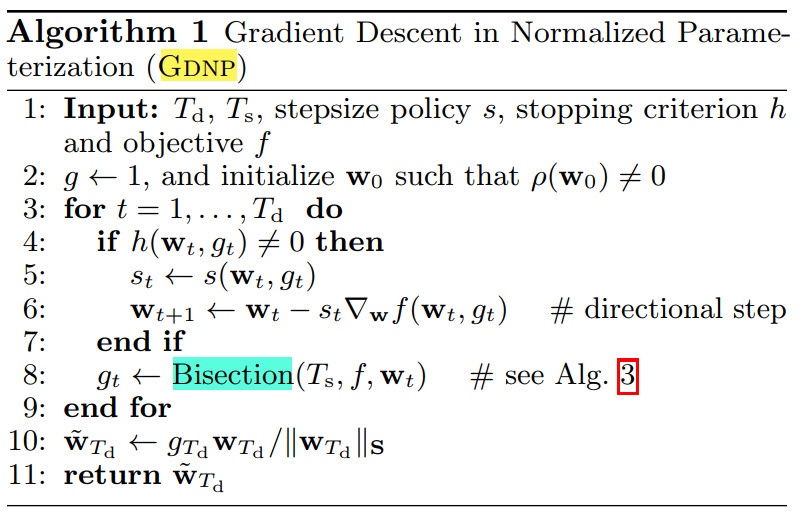
\includegraphics[scale=0.38]{pics/batchNorm/decoupling_alg1.jpg} & 
  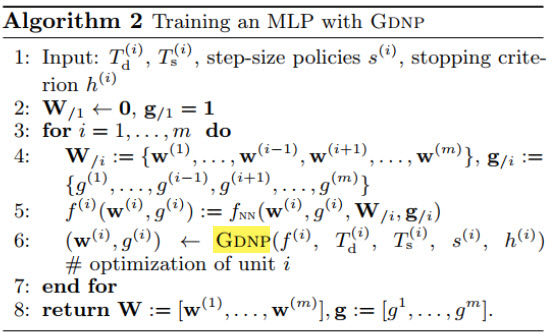
\includegraphics[scale=0.58]{pics/batchNorm/decoupling_alg2.jpg}
  \\
(1) GDNP Algorithm & (2) Training MLP with GNDP\\[6pt]
\multicolumn{2}{c}{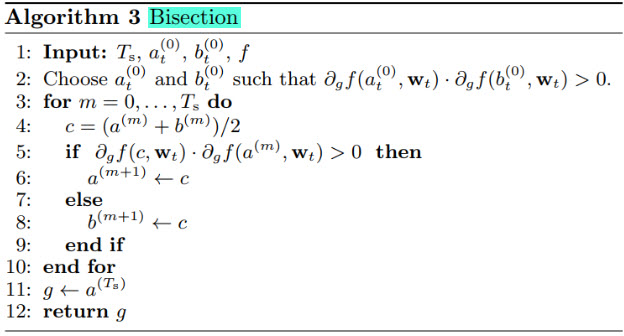
\includegraphics[scale=0.6]{pics/batchNorm/decoupling_alg3.jpg} }\\
\multicolumn{2}{c}{(3) Bisection Algorithm }
\end{tabular}
\caption{Training Algorithm}
\label{fig:algorithms}
\end{figure}

Next, they propose a training algorithm for analysis purpose, shown in Figure \ref{fig:algorithms}. The algorithm optimizes each neuron independently and sequentially (in an order of given neuron indexes). The algorithm also leverages the above \textbf{Lemma 2} decoupling input and output of an unit. Then they prove that, if all four assumptions hold, by training with the proposed algorithm (GDNP), an exponential convergence rate can be achieved:

\begin{align*}
    ||\nabla_{\Tilde{\textbf{w}}^{(i)}}f\big(\Tilde{\textbf{w}}_t^{(i)}\big)||^2_{\textbf{S}^{-1}}&\leq(1-\mu/L)^{2t}C(\rho(\textbf{w}_0)-\rho(\textbf{w}^*))+2^{-T_s^{(i)}}\zeta|b_t^{(0)}-a_t^{(0)}|/\mu^2\\\\
    \mathrm{, where\ }\Tilde{\textbf{w}}:&=g\frac{\textbf{w}}{||\textbf{w}||_{\textbf{S}}} \mathrm{\ and\ step\ size\ } s_t^{(i)}=||\textbf{w}_i^{(i)}||^3_{\textbf{S}}/(L\theta^{(i)}g_t^{(i)}\xi_t\textbf{u}^T\textbf{w}_t^{(i)})\\
    \zeta\mathrm{\ is\ }&\mathrm{Lipschitz\ constant\ of\ }f\\\\
    C&=2\Phi^2+2i\sum_{j<i}(\theta^{(j)}c_j)^2>0\\
    \rho(\textbf{w}):&=-\frac{\textbf{w}^T\textbf{uu}^T\textbf{w}}{\textbf{w}^T\textbf{Sw}}\\\\
    \xi_t&=\alpha_t^{(i)}+\sum_{j,i}\gamma_t^{(i,j)}c_j\\
    \alpha^{(i)}:&=\mathbb{E}_{\textbf{z}}\Big[l^{(1)}(F(\textbf{z},\Tilde{\textbf{W}}))\varphi^{(1)}(\textbf{z}^T\Tilde{\textbf{w}}^{(i)})\Big]-\sum_{j=1}^m\gamma^{(i,j)}(\textbf{u}^T\Tilde{\textbf{w}}^{(j)})\\
    \beta^{(i)}:&=\mathbb{E}_{\textbf{z}}\Big[l^{(1)}(F(\textbf{z},\Tilde{\textbf{W}}))\varphi^{(2)}(\textbf{z}^T\Tilde{\textbf{w}}^{(i)})\Big]\\
    \gamma^{(i,j)}:&=\theta^{(j)}\mathbb{E}_{\textbf{z}}\big[l^{(2)}(F(\textbf{z},\Tilde{\textbf{W}}))\varphi^{(1)}(\textbf{z}^T\Tilde{\textbf{w}}^{(i)})\varphi^{(1)}(\textbf{z}^T\Tilde{\textbf{w}}^{(j)})\big]\\
    \Tilde{\textbf{W}}:&=\{\Tilde{\textbf{w}}^{(1)},\cdots,\Tilde{\textbf{w}}^{(m)}\}
\end{align*}

When updating current weight parameters $(\textbf{w}^{(i)}, g^{(i)})$, they further assume that all updated neurons weights, $\{\textbf{w}^{(k)}\}_{k<i}$, are at critical points and neurons to be updated all have weight $\textbf{w}^{(k)}=\textbf{0}$ for $k>i$.

\begin{comment}
Based on the fact that

\begin{align*}
    ||\nabla_{\Tilde{\textbf{w}}^{(i)}}f\big(\Tilde{\textbf{w}}_t^{(i)}\big)||^2_{\textbf{S}^{-1}} &= ||\textbf{w}_t^{(i)}||^2_{\textbf{S}}||\nabla_{\textbf{w}^{(i)}}f(\textbf{w}_t^{(i)},g^{(i)})||^2_{\textbf{S}^{-1}}/(g_t^{(i)})^2\\
    &+\Big(\partial_{g^{(i)}}f(\textbf{w}_t^{(i)},g^{(i)}_{t})\Big)^2
\end{align*}
\end{comment}
The above convergence result is actually a composition of two parts in below: convergence of scalar $g$ and the direction $\textbf{w}$. Note that both of the two parts have exponential convergence rate.

\textbf{Convergence of scalar} $g^{(i)}$:

\begin{align*}
    \Big(\partial_{g^{(i)}}f(\textbf{w}_t^{(i)},g^{(i)}_{T_s})\Big)^2\leq2^{-T_s^{(i)}}\zeta|b_t^{(0)}-a_t^{(0)}|/\mu^2
\end{align*}

\textbf{Convergence of the direction} $\textbf{w}^{(i)}$:

\begin{align*}
    ||\textbf{w}_t^{(i)}||^2_{\textbf{S}}||\nabla_{\textbf{w}^{(i)}}f(\textbf{w}_t^{(i)},g_t^{(i)})||^2_{\textbf{S}^{-1}}\leq (1-\mu/L)^{2t}\xi_t^{2}g_t^{2}(\rho(\textbf{w}_0)-\rho(\textbf{w}^*))\\
\end{align*}

\subsubsection{Experiment}

In the experiment section, they train a neuron network of 6 hidden layers with 50 neurons each on CIFAR-10 image classification data. Note that the input data is no longer multivariate-Gaussian variables. All hidden layers are batch-normalized. For comparison, they also train an un-normalized network of the same structure. Both networks are trained by standard gradient descent and use tanh as middle layers activation. To validate \textbf{Lemma 2} that direction of critical points is independent of downstream layers, they calculate Frobenius norm of $\frac{\partial^2f_{NN}}{\partial\textbf{W}_4\partial\textbf{W}_i}$ as a measurement of cross-dependency of layer-4 with other layer, layer-$i$. Their experimental results are shown in Figure \ref{fig:decouplingexperiment}. The top two graphs clearly shows that BatchNorm network do achieve faster convergence rate. Also, the bottom two graphs shows that in BatchNorm network, dependence of a middle layer on its downstream layers (layer-5 and layer-6) becomes weaker as the layer is further away from it.

\begin{figure} 
	\centering
    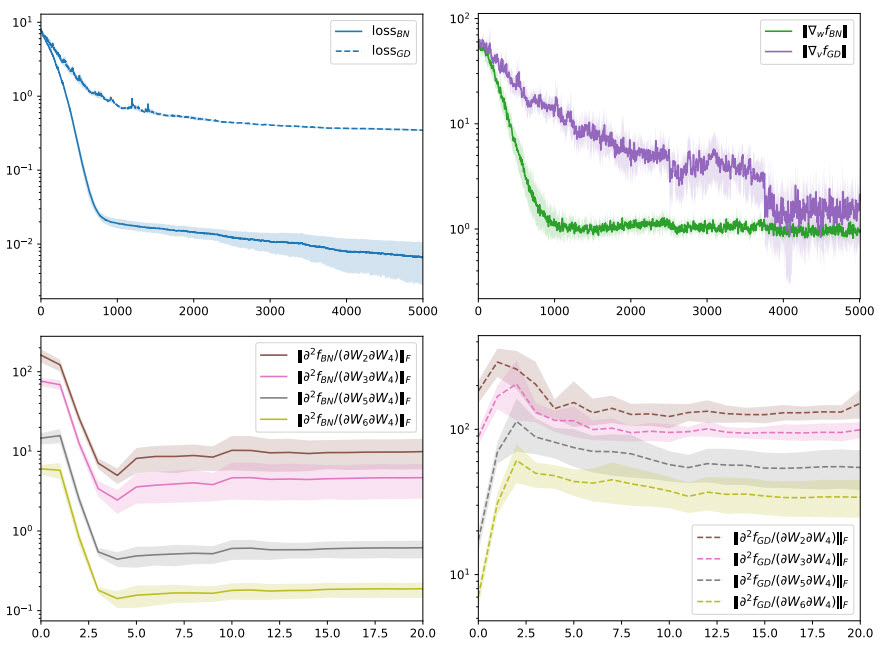
\includegraphics[width=\textwidth]{pics/batchNorm/decoupling_experiment.jpg}
	\caption{Experimental Results: Top two plots show the results of decay of loss function and norm of the loss gradient. Bottom two plots show cross-dependency in BatchNorm network and un-normalized network, respectively.}
	\label{fig:decouplingexperiment}
\end{figure}

\subsubsection{Discussion}

As for the four assumptions, the first one is feasible when input data subtracted from its mean. Assumption 2 evidently does not always hold. However, in the experiment that using non-Gaussian data, they show that the results are still valid. Assumption 3 is valid for tanh and sigmoid activations. ReLu is not differentiable at 0. However, the probability that a point is exactly zero is provable zero. Therefore, Assumption 3 is also feasible for the three enumerated popular activation functions. Last, validity of Assumption 4 is due to further proof. 

\subsection{Variants to Batch Normalization}

\subsubsection{Limitations of Batch Normalization}

Although BatchNorm is a powerful technique that speed up training process, it still has its own limitations. The mean and variance of each neuron in BatchNorm depends on size of min-batch and vary from mini-batch to min-batch. That would introduce certain amount of errors and propagate through the network which is harmful to noise sensitive applications like reinforcement learning \cite{reparameter}. Also, variance of the estimated population mean and variance is increased when mini-batch size is small. Therefore, when applying BatchNorm, the choice of mini-batch size should be considered carefully. Moreover, BatchNorm is not suitable for recurrent model like RNNs which limits application of such powerful technique.

\subsubsection{Weight Normalization}
Paper \cite{reparameter} proposed Weight Normalization (WeightNorm), another way of neural network parameterization. In their paper, weight vector is expressed as:

\begin{align*}
    \textbf{w}=\frac{g}{||\textbf{v}||}\textbf{v}
\end{align*}

where $g$ is a scalar, $\textbf{v}$ is a vector and $||\textbf{v}||$ is $l_2$ norm of $\textbf{v}$. Gradient of loss function $l$  for a WeightNorm network with respect to the new parameters $g$ and $\textbf{v}$ is:

\begin{align*}
    \nabla_gl &= \frac{\nabla_{\textbf{w}}l\cdot\textbf{v}}{||\textbf{v}||}\\
    \nabla_{\textbf{v}}l &= \frac{g}{||\textbf{v}||}\nabla_{\textbf{w}}l-\frac{g\nabla_gl}{||\textbf{v}||^2}\textbf{v}
\end{align*}

They also propose a "Mean-only" Batch Normalization adopted into the WeightNorm method by which pre-activation $t=\textbf{W}\cdot\textbf{x}$ is subtracted from its mean (without scaled by its standard deviation) then applied to non-linear activation $y=\phi(t-\mu[t])$. Parameter $\textbf{w}$ is written as WeightNorm expression. The "Mean-only" BatchNorm has an effect of centering gradient which is a low-cost operation. It their experiments, "Mean-only" WeightNorm achieves lowest test error among WeightNorm, BatchNorm and regular parameterization on a CNN network. They also apply regular WeightNorm to deep convolutional variantional auto-encoders (CVAEs), a recurrent variational autoencoder with generative model DRAW and  a Deep Q-Network (DQN) for reinforcement learning. In all three models, WeightNorm outperform normal parameterization in terms of both convergence rate and evaluation metric.

\subsubsection{Layer Normalization}
Paper \cite{layernorm} propose Layer Normalization (LayerNorm) that can be applied to recurrent-type network. Figure \ref{fig:batchvslayernorm} shows a comparison of BatchNorm and LayerNorm.  In an arbitrary layer, LayerNorm is applied on each input independently. 

\begin{figure}[h]
	\centering
    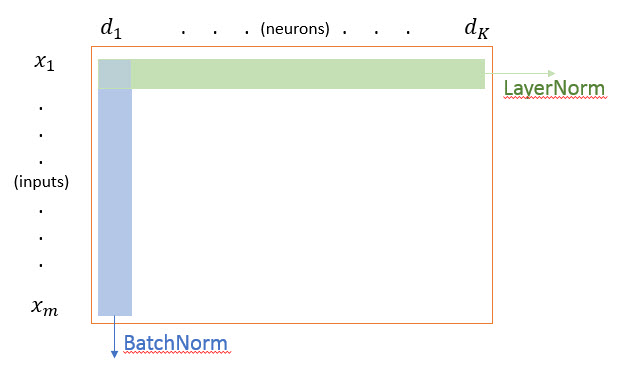
\includegraphics[scale=0.5]{pics/batchNorm/BatchNorm_vs_LayerNorm.jpg}
	\caption{Batch Normalization vs. Layer Normalization}
	\label{fig:batchvslayernorm}
\end{figure}

In a standard RNN, at time-step $t$ suppose current input $\textbf{x}^t$ and previous hidden state output $\textbf{h}^{t-1}$, let $\textbf{a}^t \in \mathbb{R}^K = W_{hh}\textbf{h}^{t-1}+W_{xh}\textbf{x}^t$, then output $\textbf{h}^t$ can be expressed as:

\begin{align*}
    \textbf{h}^t&=\sigma\Big(\frac{\textbf{g}}{\sigma^t}\odot(\textbf{a}^t - \mu^t) + \textbf{b}\Big)\\
    \mu^t&=\frac{1}{K}\sum_{i=1}^Ka_i^t\\
    \sigma^t&=\sqrt{\frac{1}{K}\sum_{i=1}^K(a_i^t-\mu^t)^2}
\end{align*}

They test with layer normalization on 5 tasks implementing RNNs. All 5 tasks converge faster than baseline model with at least comparable results (LayerNorm perform better on 3 of the 5 tasks).

\subsubsection{Group Normalization}

Small mini-batch size rapidly increases BatchNorm’s error due to inaccurate estimation of statistics. Thus, applying BatchNorm in large memory-consuming models such as computer vision tasks is limited especially for image detection, segmentation, and video classification. 

Paper \cite{groupnorm} propose Group Normalization (GroupNorm) which is independent of mini-batch size to address this issue. Implementation of GroupNorm is shown in Figure \ref{fig:groupnorm}. Calculation of the mean and variance is on each individual input across entire height and width of subset of channels in a layer. The formulation is in the same form as BatchNorm with the difference is the terms that being summed over. 

\begin{figure}[h]
	\centering
    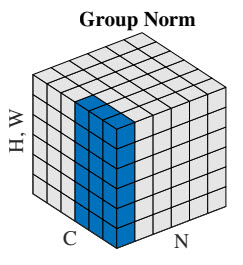
\includegraphics[scale=0.7]{pics/batchNorm/GroupNorm.jpg}
	\caption{Group Normalization: N - Mini-batch size; C - number of channels, H,W - height \& width of a feature map being flatten. Normalization is taken over the blue region.}
	\label{fig:groupnorm}
\end{figure}

Figure \ref{fig:resnet} shows the dependence of BatchNorm's performance on mini-batch size while GroupNorm doesn't have such dependence. The performance of GroupNorm is comparable as BatchNorm with larger mini-batch sizes. As for number of channels per group, they show that in ResNet-50 performance are well for all values that are studied from 2 to 64. The value can also vary from layer to layer which is another flexibility of GroupNorm.

\begin{figure}[h]
	\centering
    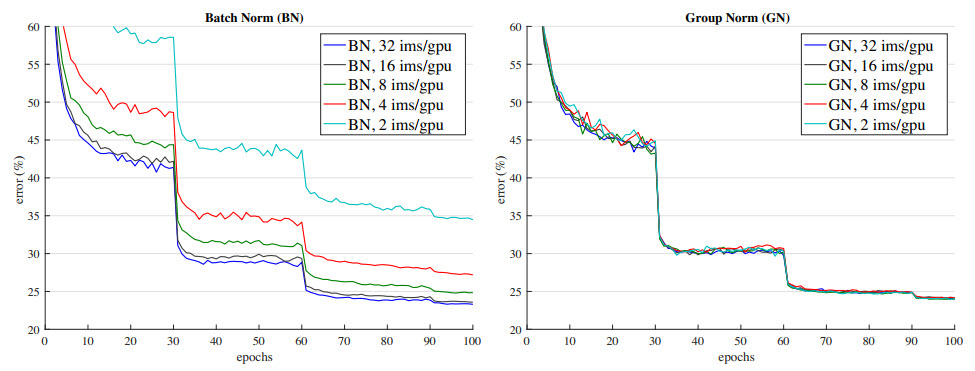
\includegraphics[scale=0.57]{pics/batchNorm/GroupNorm_vs_BatchNorm.jpg}
	\caption{ResNet-50 trained on ImageNet set}
	\label{fig:resnet}
\end{figure}

\subsubsection{Summary}
Table~\ref{normsum} shows a summary of all mentioned normalization methods along with their applications and way of calculation.\\

\begingroup
\setlength{\tabcolsep}{10pt} % Default value: 6pt
\renewcommand{\arraystretch}{1.5} % Default value: 1
\begin{table}[h] 
\centering
 \begin{tabular}{|m{10em} | m{10em} | m{10em}|} 
 \hline
 Method & Application & Calculation\\  
 \hline
 Batch Normalization & Fully Connected Layers & Individual Neuron, over mini-batch input\\ [0.5ex] 
 \hline
 Layer Normalization & Recurrent Layers & Individual Input, over all neurons in a layer\\ [0.5ex]
 \hline
 Group Normalization & Convolution Layers & Individual Input, over entire height \& weight in a group of channels\\[0.5ex]
 \hline
 Weight Normalization & Any Architecture & Decouple length and direction of weights\\
 \hline
\end{tabular}
\caption{Summary of Normalization}
\label{normsum}
\end{table}
\endgroup

\subsection{Our Own Experiments}
The first experiment conducted is a 4-layer fully connected feed-forward network with 32-64-32 neurons in each hidden layer. Output layer is a softmax layer of 10 neurons. Dataset is fashion-mnist, $28\times28$ grey scale pictures of 10 categories. BatchNorm is added to all three hidden layers as our BatchNorm network.

To verify weather Lipschitzness of the loss landscape is improved by BatchNorm as stated in Section \ref{landsmooth}, we plot the maximum loss gradient norm among batches with respect to the second last layer (calculating loss gradient norm over the entire weight space would require enormous amount of computation time, so for simplicity the calculation is only taken over one layer), shown in Figure \ref{fig:maxgradient}. The simple network architecture converges fast and later epochs indicates overfitting. So only the early epochs is presented in the graph. The top two graphs using Relu activation show that BatchNorm network has smaller gradient norm than "vanilla" network. However, the bottom two show that BatchNorm network using Tanh activation has higher gradient norm. It worth noting that results are consistent regardless of combination of learning rate and weight initialization of our choice.

\begin{figure}[h]
\begin{tabular}{cc}
  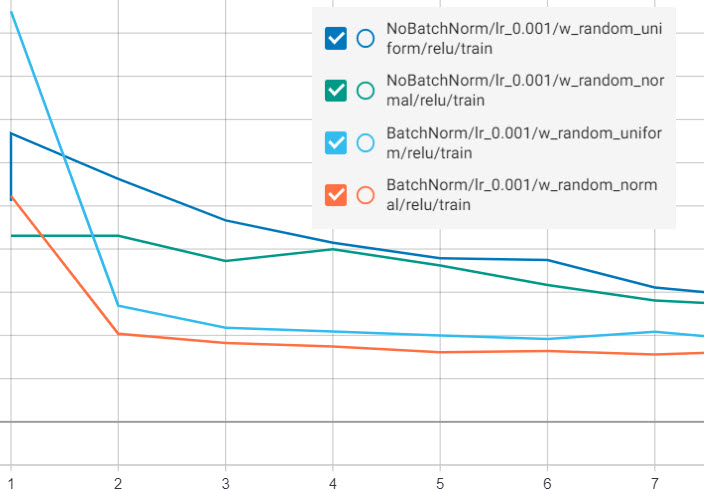
\includegraphics[scale=0.48]{pics/batchNorm/BatchNorm_relu_1.jpg} &
  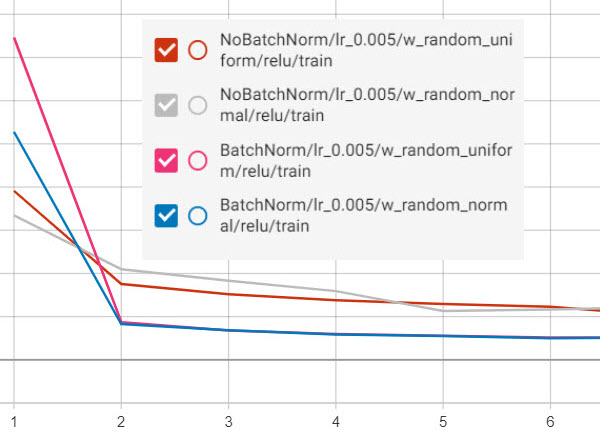
\includegraphics[scale=0.52]{pics/batchNorm/BatchNorm_relu_5.jpg}
  \\
  (1) Learning Rate=1e-3, Relu & (2) Learning Rate=5e-3, Relu\\[6pt]
  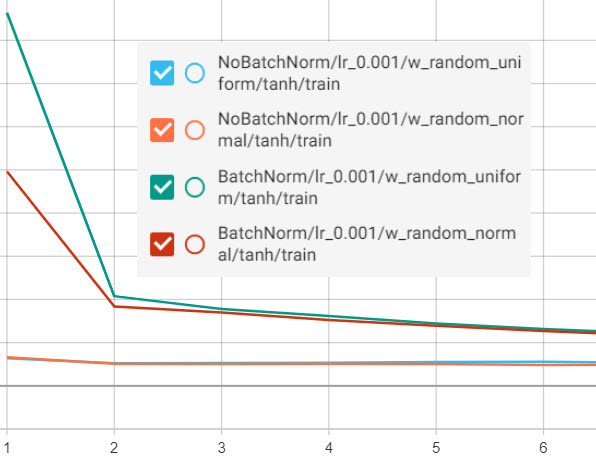
\includegraphics[scale=0.5]{pics/batchNorm/BatchNorm_tanh_1.jpg} &
  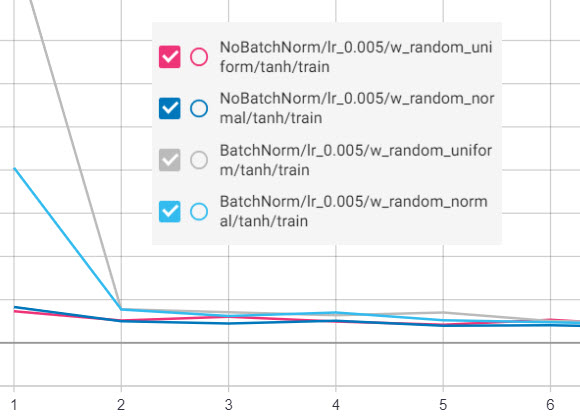
\includegraphics[scale=0.5]{pics/batchNorm/BatchNorm_tanh_5.jpg}\\
  (3) Learning Rate=1e-3, Tanh & (4) Learning Rate=5e-3, Tanh\\[6pt]
\end{tabular}
\caption{Maximum gradient norm among batches w.r.t. $W$ in last dense layer. Legend in each graph shows if BatchNorm is applied in the network, learning rate, weight initialization method and activation function. The same random seed for weight initialization is used across all runs to ensure a better control of the experiments.}
\label{fig:maxgradient}
\end{figure}

Looking again at the theory setup in Section \ref{landsmooth}, notice that output of a neuron is $y=Wx$ which omits non-linear activation function. However, if Relu is used as activation function, it can be seen as a linear calculation on positive $Wx$. For negative $Wx$, the gradient on the corresponding $W$ is zero, so those weights will not contribute to norm calculation. Therefore, gradient norm in a Relu layer is expected to satisfy \textbf{Theorem 4.4} . This conjecture can be verified on the top two graphs of Figure \ref{fig:maxgradient}. 

On the other hand, Tanh activation function can not be seen as a linear calculation. Its derivative is more complicated, therefore we cannot compare the gradient norm of a Tanh network with a linear network. It's an explanation that the behaviour of the bottom two graphs does not align with the theory.

Another observation is that the training time of BatchNorm network is twice as much as the regular network. When training a high-capacity network, since it's been observed in other papers' experiments that BatchNorm reduces the training epochs by a factor much larger than 2, the overall training speed is expected to be effectively improved by BatchNorm.

\newpage

\medskip

\small

\begin{thebibliography}{9}
\bibitem{batchnorm} 
S. Ioffe \& C. Szegedy (2015) Batch Normalization: Accelerating Deep Network Training by Reducing Internal Covariate Shift \textit{ICML}
 
\bibitem{landscape} 
S. Santurkar, D. Tsipras, A.Ilyas \& A. Madry (2018) How Does Batch Normalization Help Optimization? \textit{32nd Conference on In NeurIPS}

\bibitem{dln} 
A. M. Saxe, J. Mcclelland \& S. Ganguli (2014). Exact solutions to the nonlinear dynamics of learning in deep linear neural networks.
 
\bibitem{decoupling} 
J. Kohler, H. Daneshmand, A. Lucchi et. al. (2019) Exponential convergence rates for Batch Normalization:The power of length-direction decoupling in non-convex optimization. 	\textit{Proceedings of Machine Learning Research, PMLR 89:806-815.}

\bibitem{reparameter}
T. Salimans \& D.P. Kingma. (2016) Weight normalization: A simple reparameterization to accelerate
training of deep neural networks. \textit{In Advances in Neural Information Processing Systems (NIPS)}.

\bibitem{layernorm}
J.L. Ba, J.R Kiros \& G.E Hinton (2016) Layer Normalization. \textit{arXiv:1607.06450}

\bibitem{groupnorm}
Y. Wu \& K. He (2018) Group Normalization \textit{European Conference on Computer Vision (ECCV)}

\bibitem{Milman}
Milman, V. D., \& Schechtman, G. (2009). \textit{Asymptotic theory of finite dimensional normed spaces: Isoperimetric inequalities in Riemannian manifolds} (Vol. 1200). Springer.

\bibitem{chen}
Chen, L., Wang, H., Zhao, J., Papailiopoulos, D., \& Koutris, P. (2018). \textit{The effect of network width on the performance of large-batch }. In Advances in Neural Information Processing Systems (pp. 9302-9309).

\bibitem{dong}
Yin, D., Pananjady, A., Lam, M., Papailiopoulos, D., Ramchandran, K., \& Bartlett, P. (2017). \textit{Gradient diversity: a key ingredient for scalable distributed learning}. arXiv preprint arXiv:1706.05699.

\bibitem{SimonDu}
Simon S.Du,X.Zhai.,B. Poczos.,A.Singh.(2019).\textit{Gradient Descent Provably Optimizes Over-parameterized Neural Networks}

\bibitem{Arora}
S.Arora, Simon S.Du, W.Hu ,Z.Li.,R.Wang(2019).\textit{Fine-Grained Analysis of Optimization and Generalization for Overparameterized Two-Layer Neural Networks}

\bibitem{SoudryCarmon}
D.Soudry, Y.Carmon(2016).\textit{No bad local minima:Data independent training error guarantees for multilayer neural networks}

\bibitem{Weinan1}
Weinan.E, Chao M.,Lei W.(2019).\textit{A Priori Estimates For Two-layer Neural Networks}

\bibitem{Weinan2}
Weinan.E, Chao M.,Lei W.(2019).\textit{A Comparative Analysis of the Optimization and Generalization Property of Two-layer Neural Network and Random Feature Models Under Gradient Descent Dynamics}

\bibitem{oymak}
Oymak, S., \& Soltanolkotabi, M. (2018). Overparameterized Nonlinear Learning: Gradient Descent Takes the Shortest Path?. arXiv preprint arXiv:1812.10004.

\bibitem{bassily}
Bassily, R., Belkin, M., \& Ma, S. (2018). \textit{On exponential convergence of SGD in non-convex over-parametrized learning}. arXiv preprint arXiv:1811.02564.

\bibitem{gradient_confusion}
Sankararaman, K. A., De, S., Xu, Z., Huang, W. R., \& Goldstein, T. (2019). \textit{The Impact of Neural Network Overparameterization on Gradient Confusion and Stochastic Gradient Descent}. arXiv preprint arXiv:1904.06963.

\end{thebibliography}






\end{document}

